\section{Motivation}

DAS
Big Data Processing
Anomaly Detection 
Unsupervised (v supervised and smaller models)
CGF (Tools and Resources)
What we have available

Recorded \acrshort{das} signals has the potential to become quite large, taking up a large amount of computer memory. Improving methods for storing reduced To process these data, parallel techniques have the ability to drastically reduce the overall runtime, utilizing as many ... . Furthermore, 


\subsection{Anomaly Detection}

Traditionally, clustering based \acrfull{ml} techniques such as K-MEANS, DBSCAN and HDBSCAN have been quite popular for anomaly detection. However, these methods often require manual feature engineering, require labeled datasets or generally do not scale to large datasets. 

\begin{figure}[ht]
    \centering
    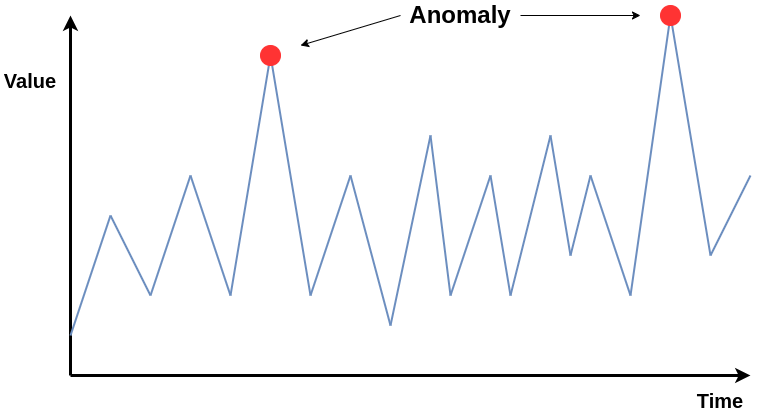
\includegraphics[scale=0.4]{figures/anolay_line.png}
    \caption{Example of anomalies in a dataset}
    \label{fig:anomaly_example}
\end{figure}


\subsection{Autoencoders for Anomaly Detection}

However, with the upcoming of \acrshort{das}, both unsupervised and supervised \acrfull{dl} methods have proven to produce even better results for anomaly detection. For \acrshort{das} data specifically, both scalability and manual labeling can become quite tedious, or outright non-feasible. For 

Unsupervised learning has in later years returned after the explosion of generative models [CITE]. Compared to their supervised alternatives, unsupervised do not require manual labeling. They're therefore not prone to some of the more common problems within supervised methods, such as detecting irregular events.   are well suited for detecting novel anomalies \cite{wei2022lstmautoencoder, srivastava2016unsupervised} compared to its supervised alternatives, and do not require manual labeling. This makes them 

Current autoencoder based approaches to anomaly detection of \acrshort{das} do not emphasize the overall memory consumption as well as the convertion of models to a real-time environment. This 

\acrshort{das} technology in itself has now started garnering attention for research, and several papers have previously studied  how one can process this data. \acrshort{ai} and \acrshort{ml} models have been constructed for looking at time series data, and analyzing sensor data, although several of theses have studied .  Only recently has \acrshort{ai}

Previous work on this data \cite{projthesis} revolved around processing \acrshort{hdf5} files as fast and efficient as possible, trying to parallellize already existent code, and take advantage of newer technologies, such as Julia.

\subsection{Current Tools at \acrshort{cgf}}

\acrfull{cgf} spend a lot of time and resources on processing and analysing \acrshort{das} data. Current tools for processing are quite slow, and do not utilize parallelization techniques that has the potential to drastically speed up computations. Additionally, analysis is often done using more traditional signal processing techniques, not leveraging the potential benefits of more novel \acrshort{ann} methods. \\ \\  

We hereby present two programs: Judas and TinyDAS. Judas is a package consisting of methods for parsing \acrshort{das} data stored in \acrfull{hdf5} files,  processing them in a parallel manner. TinyDAS is a Python program for training autoencoder models and detecting anomalies , with a potential for real-time analysis. Combined, these two packages aims at expanding current tools available at \acrshort{cgf} for processing and analysing \acrshort{das} data. To evaluate our work, we use both proprietary and open source data. 

\begin{figure}[h]
    \centering
    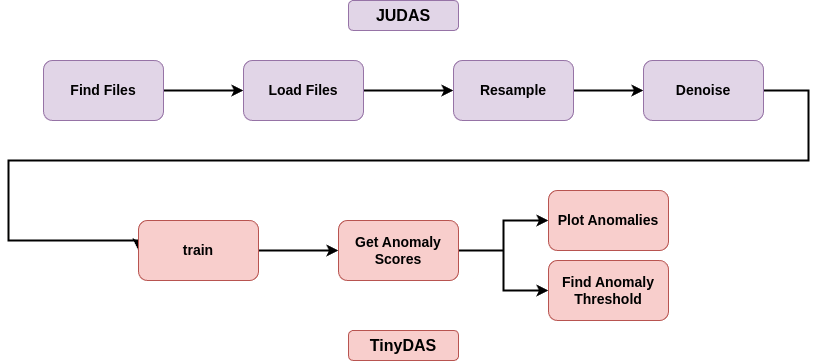
\includegraphics[scale=.5]{figures/api_overview.png}
    \caption{JudasNET Api overview}
    \label{fig:judasnet_overview}
\end{figure}